\documentclass{ximera}
\graphicspath{  %% When looking for images,
{./}            %% look here first,
{./pictures/}   %% then look for a pictures folder,
{../pictures/}  %% which may be a directory up.
{../../pictures/}  %% which may be a directory up.
{../../../pictures/}  %% which may be a directory up.
{../../../../pictures/}  %% which may be a directory up.
}

\usepackage{listings}
\usepackage{circuitikz}
\usepackage{xcolor}
\usepackage{amsmath,amsthm}
\usepackage{subcaption}
\usepackage{graphicx}
\usepackage{tikz}
\usepackage{tikz-3dplot}
\usepackage{amsfonts}
\usepackage{mdframed} % For framing content
\usepackage{tikz-cd}

  \renewcommand{\vector}[1]{\left\langle #1\right\rangle}
  \newcommand{\arrowvec}[1]{{\overset{\rightharpoonup}{#1}}}
  \newcommand{\ro}{\texttt{R}}%% row operation
  \newcommand{\dotp}{\bullet}%% dot product
  \renewcommand{\l}{\ell}
  \let\defaultAnswerFormat\answerFormatBoxed
  \usetikzlibrary{calc,bending}
  \tikzset{>=stealth}
  




%make a maroon color
\definecolor{maroon}{RGB}{128,0,0}
%make a dark blue color
\definecolor{darkblue}{RGB}{0,0,139}
%define the color fourier0 to be the maroon color
\definecolor{fourier0}{RGB}{128,0,0}
%define the color fourier1 to be the dark blue color
\definecolor{fourier1}{RGB}{0,0,139}
%define the color fourier 1t to be the light blue color
\definecolor{fourier1t}{RGB}{173,216,230}
%define the color fourier2 to be the dark green color
\definecolor{fourier2}{RGB}{0,100,0}
%define teh color fourier2t to be the light green color
\definecolor{fourier2t}{RGB}{144,238,144}
%define the color fourier3 to be the dark purple color
\definecolor{fourier3}{RGB}{128,0,128}
%define the color fourier3t to be the light purple color
\definecolor{fourier3t}{RGB}{221,160,221}
%define the color fourier0t to be the red color
\definecolor{fourier0t}{RGB}{255,0,0}
%define the color fourier4 to be the orange color
\definecolor{fourier4}{RGB}{255,165,0}
%define the color fourier4t to be the darker orange color
\definecolor{fourier4t}{RGB}{255,215,0}
%define the color fourier5 to be the yellow color
\definecolor{fourier5}{RGB}{255,255,0}
%define the color fourier5t to be the darker yellow color
\definecolor{fourier5t}{RGB}{255,255,100}
%define the color fourier6 to be the green color
\definecolor{fourier6}{RGB}{0,128,0}
%define the color fourier6t to be the darker green color
\definecolor{fourier6t}{RGB}{0,255,0}

%New commands for this doc for errors in copying
\newcommand{\eigenvar}{\lambda}
%\newcommand{\vect}[1]{\mathbf{#1}}
\renewcommand{\th}{^{\text{th}}}
\newcommand{\st}{^{\text{st}}}
\newcommand{\nd}{^{\text{nd}}}
\newcommand{\rd}{^{\text{rd}}}
\newcommand{\paren}[1]{\left(#1\right)}
\newcommand{\abs}[1]{\left|#1\right|}
\newcommand{\R}{\mathbb{R}}
\newcommand{\C}{\mathbb{C}}
\newcommand{\Hilb}{\mathbb{H}}
\newcommand{\qq}[1]{\text{#1}}
\newcommand{\Z}{\mathbb{Z}}
\newcommand{\N}{\mathbb{N}}
\newcommand{\q}[1]{\text{``#1''}}
%\newcommand{\mat}[1]{\begin{bmatrix}#1\end{bmatrix}}
\newcommand{\rref}{\text{reduced row echelon form}}
\newcommand{\ef}{\text{echelon form}}
\newcommand{\ohm}{\Omega}
\newcommand{\volt}{\text{V}}
\newcommand{\amp}{\text{A}}
\newcommand{\Seq}{\textbf{Seq}}
\newcommand{\Poly}{\textbf{P}}
\renewcommand{\quad}{\text{    }}
\newcommand{\roweq}{\simeq}
\newcommand{\rowop}{\simeq}
\newcommand{\rowswap}{\leftrightarrow}
\newcommand{\Mat}{\textbf{M}}
\newcommand{\Func}{\textbf{Func}}
\newcommand{\Hw}{\textbf{Hamming weight}}
\newcommand{\Hd}{\textbf{Hamming distance}}
\newcommand{\rank}{\text{rank}}
\newcommand{\longvect}[1]{\overrightarrow{#1}}
% Define the circled command
\newcommand{\circled}[1]{%
  \tikz[baseline=(char.base)]{
    \node[shape=circle,draw,inner sep=2pt,red,fill=red!20,text=black] (char) {#1};}%
}

% Define custom command \strikeh that just puts red text on the 2nd argument
\newcommand{\strikeh}[2]{\textcolor{red}{#2}}

% Define custom command \strikev that just puts red text on the 2nd argument
\newcommand{\strikev}[2]{\textcolor{red}{#2}}

%more new commands for this doc for errors in copying
\newcommand{\SI}{\text{SI}}
\newcommand{\kg}{\text{kg}}
\newcommand{\m}{\text{m}}
\newcommand{\s}{\text{s}}
\newcommand{\norm}[1]{\left\|#1\right\|}
\newcommand{\col}{\text{col}}
\newcommand{\sspan}{\text{span}}
\newcommand{\proj}{\text{proj}}
\newcommand{\set}[1]{\left\{#1\right\}}
\newcommand{\degC}{^\circ\text{C}}
\newcommand{\centroid}[1]{\overline{#1}}
\newcommand{\dotprod}{\boldsymbol{\cdot}}
%\newcommand{\coord}[1]{\begin{bmatrix}#1\end{bmatrix}}
\newcommand{\iprod}[1]{\langle #1 \rangle}
\newcommand{\adjoint}{^{*}}
\newcommand{\conjugate}[1]{\overline{#1}}
\newcommand{\eigenvarA}{\lambda}
\newcommand{\eigenvarB}{\mu}
\newcommand{\orth}{\perp}
\newcommand{\bigbracket}[1]{\left[#1\right]}
\newcommand{\textiff}{\text{ if and only if }}
\newcommand{\adj}{\text{adj}}
\newcommand{\ijth}{\emph{ij}^\text{th}}
\newcommand{\minor}[2]{M_{#2}}
\newcommand{\cofactor}{\text{C}}
\newcommand{\shift}{\textbf{shift}}
\newcommand{\startmat}[1]{
  \left[\begin{array}{#1}
}
\newcommand{\stopmat}{\end{array}\right]}
%a command to give a name to explorations and hints and theorems
\newcommand{\name}[1]{\begin{centering}\textbf{#1}\end{centering}}
\newcommand{\vect}[1]{\vec{#1}}
\newcommand{\dfn}[1]{\textbf{#1}}
\newcommand{\transpose}{\mathsf{T}}
\newcommand{\mtlb}[2][black]{\texttt{\textcolor{#1}{#2}}}
\newcommand{\RR}{\mathbb{R}} % Real numbers
\newcommand{\id}{\text{id}}

\author{Zack Reed} %PEter Selinger
\title{Systems of Equations and Applications}
\begin{document}
\begin{abstract}
Here we introduce one of the most prevalent applications of matrices and vectors, the solving of systems of equations.
\end{abstract}
\maketitle



\tikzstyle geometryDiagrams=[ultra thick,color=blue!50!black]

\section{Matrix-Vector Products Yield Systems of Equations}

Systems of linear equations are everywhere, and one of the key applications of vectors and matrices is the efficient solving of such systems. Let's begin with an example from circuits!

\begin{exploration}\name{Circuit Analysis and Systems of Equations}

  The tools of linear algebra can be used to study the application of resistor networks. 

There is a difference in electric potential between the $+$ and $-$ terminals of a battery, measured in volts. This difference in potential causes a current to flow through a circuit. The current is measured in amperes (amount of charge per second) and is slowed by resistors in the circuit. 

An example of an electrical circuit is below.

\begin{center}
  %\scalebox{0.8}{
  %  \begin{circuitikz}[american] \draw
  %    (0,0) to [battery1, v^= $18\volt$~~] (0,4)
  %    (0,0) to [R = $2 \ohm$] (4,0)
  %    to [R = $4 \ohm$] (4,4)
  %    (0,4) to [R =$2 \ohm$] (4,4)
  %    (2,2) node[scale=4]{$\circlearrowleft$}
  %    (2,2) node{$I_1$}
  %    ;
  %  \end{circuitikz}
  %}
  %include image from circuit-1
  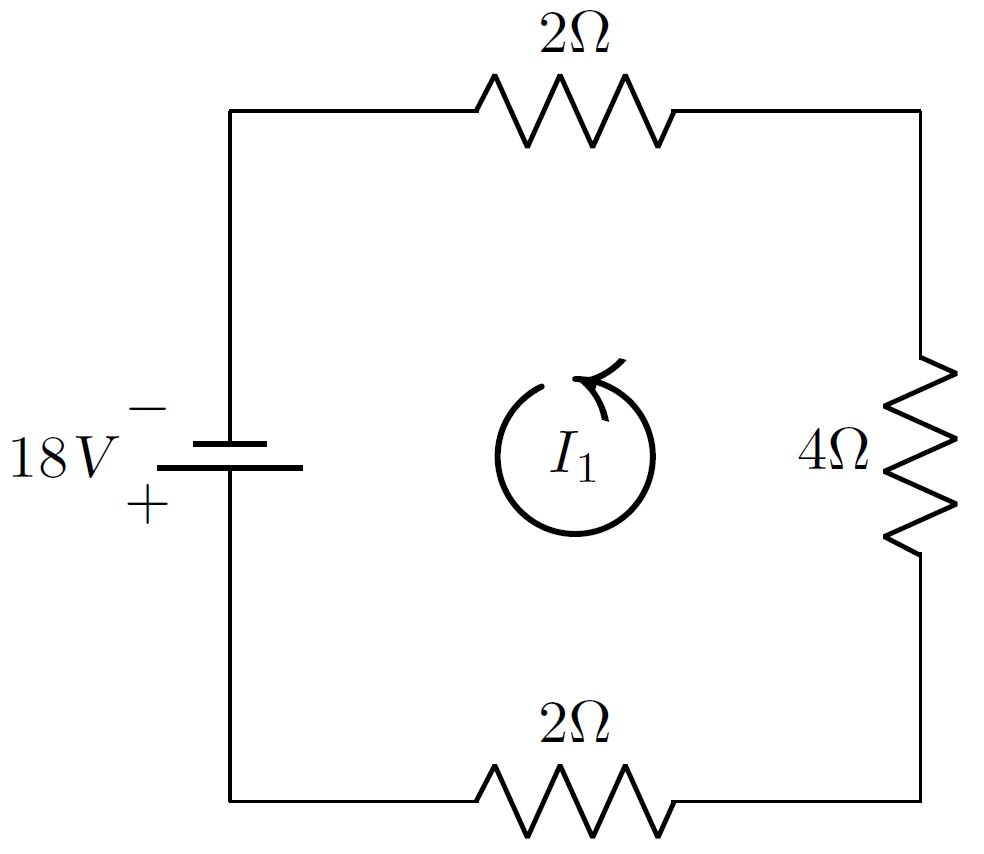
\includegraphics{circuits-1.png}
\end{center}

\noindent
The jagged lines %(\begin{circuitikz}[baseline=-0.5ex] \draw (0,0) to
  %[R] (2,0); \end {circuitikz}) 
  denote resistors and the numbers next
to them give their resistance%
\index{resistance} in ohms (i.e. volts/amperes), written as $\ohm$. The voltage%
\index{voltage} source %(\begin{circuitikz}[baseline=-0.5ex] \draw
  %(0,0) to [/tikz/circuitikz/bipoles/length=0.75cm, battery1]
  %(1,0); \end {circuitikz}) 
  causes the current%
\index{current} to flow in the direction from the longer of the two
lines toward the shorter\footnote{By {\em current}, we always mean the
  {\em conventional current}, which flows from plus to minus. It is
  the opposite of the electron flow, which goes from minus to plus.}.
Voltage is measured in volts, written as $\volt$.  The current for a
circuit is labelled $I_k$, and is measured in amperes, written as
$\amp$.

In the above figure, the current $I_1$ has been labelled with an arrow
in the counterclockwise direction. This is an entirely arbitrary
decision and we could have chosen to label the current in the
counterclockwise direction.  With our choice of direction here, we
define a positive current to flow in the counterclockwise direction
and a negative current to flow in the clockwise direction.

The goal of this section is to use the values of resistors and voltage
sources in a circuit to determine the current. An essential theorem
for this application is Kirchhoff's law%
\index{Kirchhoff's law}.

\begin{theorem}{Kirchhoff's law}{kirchhoff-law}
  The sum of the resistance ($R$) times the amperes ($I$) in the
  counterclockwise direction around a loop equals the sum of the
  voltage sources ($V$) in the same direction around the loop.
\end{theorem}

Kirchhoff's law allows us to set up a system of linear equations and
solve for any unknown variables. When setting up this system, it is
important to trace the circuit in the counterclockwise direction. If a
resistor or voltage source is crossed against this direction, the
related term must be given a negative sign.

We will explore this in the next example where we determine the value
of the current in the initial diagram.

\begin{example}\name{Solving for current}
  Applying Kirchhoff's Law to the diagram below, determine the value for $I_1$.

  \begin{center}
    %\scalebox{0.8}{
    %  \begin{circuitikz}[american,scale=0.8] \draw
    %%    (0,0) to [battery1, v^= $18\volt$~~] (0,4)
     %   (0,0) to [R = $2 \ohm$] (4,0)
     %   to [R = $4 \ohm$] (4,4)
     %   (0,4) to [R =$2 \ohm$] (4,4)
     %   (2,2) node[scale=4]{$\circlearrowleft$}
     %   (2,2) node{$I_1$}
     %   ;
     % \end{circuitikz}
    %}
    %include image from circuit-2
    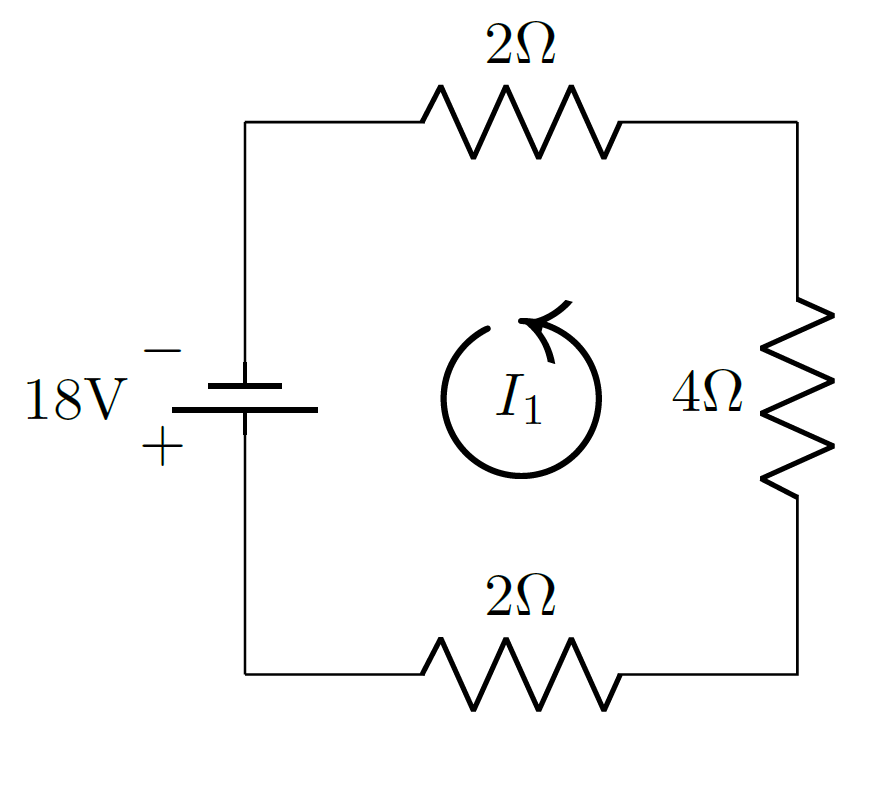
\includegraphics{circuits-2.png}
  \end{center}



\begin{solution}
  Begin in the bottom left corner, and trace the circuit in the
  counterclockwise direction. At the first resistor, multiplying
  resistance and current gives $2I_1$. Continuing in this way through
  all three resistors gives $2I_1 + 4I_1 + 2 I_1$. This must equal the
  voltage source in the same direction. Notice that the direction of
  the voltage source matches the counterclockwise direction specified,
  so the voltage is positive.

  Therefore the equation is given by
  \begin{eqnarray*}
    2I_1 + 4I_1 + 2 I_1 &=& 18, \\
  \end{eqnarray*}

  Our unknown current is $I_1$, and we can solve for $I_1$ in the usual algebraic way. The equation simplifies to

  and the solution is
  \begin{eqnarray*}
    8I_1 &=& 18, \\
    I_1 &=& \answer{9/4} \amp.
  \end{eqnarray*}
  Remember that the unit for current is $\amp$. Since the answer is positive, this confirms that the current flows
  counterclockwise.
\end{solution}

\end{example}

\begin{example}\name{Unknown currents}
  The diagram below consists of four circuits. The current ($I_k$) in
  the four circuits is denoted by $I_1$, $I_2$, $I_3$, $I_4$. Using
  Kirchhoff's Law, write an equation for each circuit and solve for
  each current.

  \begin{center}
    %\scalebox{0.8}{
    %  \begin{circuitikz}[american, scale=0.7] \draw
    %    (0,0) to [battery1, v^= $18\volt$~~] (0,4)
    %    (0,0) to [R = $2 \ohm$] (4,0)
    %    to [R = $4 \ohm$] (4,4)
    %    (0,4) to [R =$2 \ohm$] (4,4)
    %    (6,4) to [battery1, v_= \raisebox{1ex}{$27\volt$}] (4,4)
    %    (6,4) to [R = $3 \ohm$] (8,4)
    %    to [R = $1 \ohm$] (8,0)
    %    (4,0) to [R = $6 \ohm$] (8,0)
    %    to [R = $2 \ohm$] (8,-4)
    %    to [R = $3 \ohm$] (4,-4)
    %    to [R = $1 \ohm$] (4,0)
    %    (4,-4)to [R = $5 \ohm$] (0,-4)
    %    (0,0) to [battery1, v_= $23\volt$~~] (0,-4)
    %    (2,2) node[scale=3]{$\circlearrowleft$}
    %    (2,2) node{$I_2$}
    %    (6,2) node[scale=3]{$\circlearrowleft$}
    %    (6,2) node{$I_3$}
    %    (6,-2) node[scale=3]{$\circlearrowleft$}
    %    (6,-2) node{$I_4$}
    %    (2,-2) node[scale=3]{$\circlearrowleft$}
    %    (2,-2) node{$I_1$}
    %    ;
    %  \end{circuitikz}
    %}
    %include image from circuit-3
    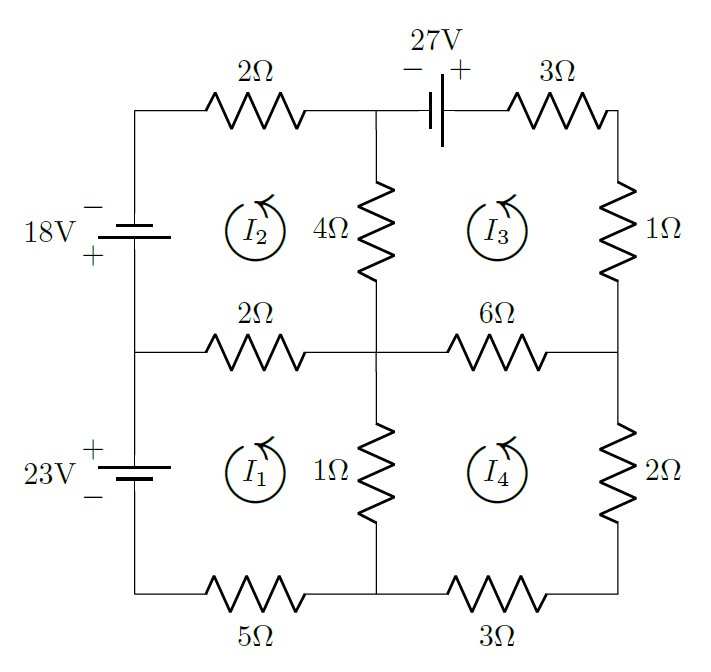
\includegraphics{circuits-3.png}
  \end{center}

  Starting with the top left circuit, multiply the resistance by the
  current and sum the resulting products. Specifically, consider the
  resistor labelled $2 \ohm$ that is part of the circuits of $I_1$ and
  $I_2$. 
  
  Notice that current $I_2$ runs through this in a positive
  (counterclockwise) direction, and $I_1$ runs through in the opposite
  (negative) direction. The product of resistance and current is then
  $2 (I_2 - I_1) = 2I_2 - 2I_1$.  
  
  Continue in this way for each
  resistor, and set the sum of the products equal to the voltage
  source to write the equation:
  \begin{equation*}
    2I_2-2I_1+4I_2-4I_3+2I_2=18.
  \end{equation*}
  The above process is used on each of the other three circuits, and
  the resulting equations are:

  \noindent
  Upper right circuit:
  \begin{equation*}
    4I_3 - 4I_2 + 6I_3 - 6I_4 + I_3 + 3I_3 = -27.
  \end{equation*}
  Lower right circuit:
  \begin{equation*}
    3I_4 + 2I_4 + 6I_4 - 6I_3 + I_4 - I_1 = 0.
  \end{equation*}
  Lower left circuit:
  \begin{equation*}
    5I_1+I_1-I_4+2I_1-2I_2=-23.
  \end{equation*}

  Notice that the voltage for the upper right and lower left circuits
  are negative due to the clockwise direction they indicate. The
  resulting system has four equations in four variables. 

  \begin{remark}

    This first example of a system of equations highlights some important assumptions that we'll make in order to utilize the tools from linear algebra.

    First, the system is complex because each equation must be satisfied simultaneously for the entire system to have a solution. We saw this briefly when examining the span of vector sets, that any solution must satisfy all equations in the system.

    Second, for the purpose of this course we're only going to consider \emph{linear} systems. In true fashion, we mean that all elements of the system must be the results of addition or scalar multiplication. This is a little different from the vector example, as technically the variables are scalars, but what we mean here is that you can only construc the system by multiplying scalars to variables, or by adding products together. 

    This brings the following definitions.

    \begin{definition}\name{Linear equation}
      A \textbf{linear equation}%
      \index{linear equation} is an equation of the form
      \begin{equation*}
        a_1x_1 + a_2x_2 + \ldots + a_nx_n = b.
      \end{equation*}
      Here, $a_1,\ldots,a_n$ are real numbers called the
      \textbf{coefficients}%
      \index{coefficient} of the equation, $b$ is a real number called the
      \textbf{constant term}%
      \index{constant term} of the equation, and $x_1,\ldots,x_n$ are
      \textbf{variables}%
      \index{variable}.
    \end{definition}

    \begin{example}{Linear vs. non-linear equation}{linear-vs-non-linear}
      Which of the following equations are linear?
      \begin{equation*}
        \begin{array}{cc}
          2x+3y=5 & is \wordChoice{\choice[correct]{linear},\choice{non linear}}\\
          2x^2+3y=5 & is \wordChoice{\choice{linear},\choice[correct]{non linear}}\\
          2\sqrt{x} + 3y = 5 & is \wordChoice{\choice{linear},\choice[correct]{non linear}}\\
          (\sqrt{2}) x + 3y = 5^2 & is \wordChoice{\choice[correct]{linear},\choice{non linear}}
        \end{array}
      \end{equation*}
    \end{example}

    We then need to define a system of linear equations.

    \begin{definition}\name{System of linear equations}
      A \textbf{system of linear equations}%
      \index{system of linear equations} is a list of equations
      \begin{equation*}
        \begin{array}{c@{~}c@{~}c}
          a_{11}x_1+a_{12}x_2+\ldots+a_{1n}x_n&=&b_1 \\
          a_{21}x_1+a_{22}x_2+\ldots+a_{2n}x_n&=&b_2 \\
          \vdots \\
          a_{m1}x_1+a_{m2}x_2+\ldots+a_{mn}x_n&=&b_m,
        \end{array}
      \end{equation*}
      where $a_{ij}$ and $b_i$ are scalars (i.e., real numbers). The above
      is a system of $m$ equations in the $n$ variables
      $x_1,x_2\ldots,x_n$.  As before, the numbers $a_{ij}$ are called the
      \textbf{coefficients}%
      \index{coefficient} and the numbers $b_i$ are called the
      \textbf{constant terms}%
      \index{constant term} of the system of equations.
    \end{definition}

    Finally, we want some terminology for whether at least one solution to a system exists.

    \begin{definition}\name{Consistent and inconsistent systems}
      A system of linear equations is called \textbf{consistent}%
      \index{consistent system}%
      \index{system of linear equations!consistent} if there exists at
      least one solution. It is called \textbf{inconsistent}%
      \index{inconsistent system}%
      \index{system of linear equations!inconsistent} if there is no
      solution.
    \end{definition}

  \end{remark}

\begin{solution}
  
  Let's now return to our linear system of equations and determine whether the system is consistent or inconsistent.

  First, rearranging and simplifying so that we list the variables in order, we have:
  \begin{equation*}
    \begin{array}{r@{~}c@{~}l}
      -2I_1+8I_2-4I_3&=&18, \\
      - 4I_2 + 14I_3 - 6I_4 &=& -27, \\
      -I_1 - 6I_3 + 12I_4 &=& 0, \\
      8I_1-2I_2 - I_4 &=& -23.
    \end{array}
  \end{equation*}

  We're going to solve the system systematically, by rearranging terms and manipulating equations so that we don't alter the solutions at all, but so that we can solve for one variable at a time. This is the same process we use when we solve simple algebraic equations, but we're going to be a little more systematic about it.

  \begin{remark}

  We first need to give ourselves some ways to manipulate the system without changing the solutions. These are called \emph{elementary row operations} (or more typically just elementary operations). The somewhat evocative use of the term \emph{row} should perk our ears to suggest that there will be an explicit connection to matrices down the road!

  \begin{definition}\name{Elementary operations}
    \textbf{Elementary operations}%
    \index{elementary operation} are the
    following operations:
  
    \begin{enumerate}
    \item Interchange the order in which the equations are listed.
  
    \item Multiply any equation by a non-zero scalar.
  
    \item Add a multiple of one equation to another equation.
    \end{enumerate}
  \end{definition}

  \end{remark}

  Let's use these elementary row operations to solve the system. Our goal is to get the system into a form where each equation only has one variable on the left, and one constant on the right. If we can make the system look like this, we'll have found our solution.

  One by one, we'll give each variable a coefficient of $1$, and then eliminate all instances of that variable from the other equations. 
  
  We'll start with $I_1$, let's multiply the first equation by $-1/2$, and then also note any terms with $0$ coefficients so that we keep track of variables more easily. We'll also write the altered equation in red so that we can keep track of our progress.

  \begin{equation*}
    \begin{array}{r@{~}c@{~}l}
      \color{red}I_1-4I_2+2I_3+0I_4&=&\color{red}-9, \\
      0I_1- 4I_2 + 14I_3 - 6I_4 &=& -27, \\
      -I_1 +0I_2 - 6I_3 + 12I_4 &=& 0, \\
      8I_1-2I_2 +0I_3 - I_4 &=& -23.
    \end{array}
  \end{equation*}

  Now, we add a multiple of the first equation to all of the other equations to eliminate $I_1$ from them. Since equation 3 has a coefficient of $-1$ for $I_1$, we'll just add the first equation to the third equation. 

  Since the fourth equation has a coefficient of $8$ for $I_1$, we'll add $-8$ times the first equation to the fourth equation.

  This gives the following system:

  \begin{equation*}
    \begin{array}{r@{~}c@{~}l}
      I_1-4I_2+2I_3+0I_4&=&-9, \\
      0I_1- 4I_2 + 14I_3 - 6I_4 &=& -27, \\
      \color{red}0I_1 - 4I_2 - 4I_3 + 12I_4 &=& \color{red}-9, \\
      \color{red}0I_1+30I_2 - 16I_3 - I_4 &=& \color{red}49.
    \end{array}
  \end{equation*}

  Here's the great part about this process: now that the last three equations have $0I1$, adding a multiple of these equations back to $I_1$ won't change the $I_1$ term, so we've now isolated $I_1$!

  Let's move to $I_2$. We'll multiply the second equation by $-1/4$ so that it has a coefficient of $1$ for $I_2$.

  \begin{equation*}
    \begin{array}{r@{~}c@{~}l}
      I_1-4I_2+2I_3+0I_4&=&-9, \\
      \color{red}0I_1+I_2 - 7/2I_3 + 3/2I_4 &=& \color{red}27/4, \\
      0I_1 - 4I_2 - 4I_3 + 12I_4 &=& -9, \\
      0I_1+30I_2 - 16I_3 - I_4 &=& 49.
    \end{array}
  \end{equation*}

  Now we eliminate $I_2$ from the remaining equations. Let's take some shorthand now to reference the row operations we're doing. We're going to change the first row by adding $4$ times the second row to it, let's denote that by $R_1 \rightarrow R_1 + 4R_2$. We then similarly alter the third and fourth rows, so we denote that by $R_3 \rightarrow R_3 + 4R_2$ and $R_4 \rightarrow R_4 - 30R_2$.

  This yields the system:

  \begin{equation*}
    \begin{array}{r@{~}c@{~}l}
      \color{red}I_1+0I_2-12I_3+6I_4&=&\color{red}18, \\
      0I_1+I_2 - 7/2I_3 + 3/2I_4 &=& 27/4, \\
      \color{red}0I_1 + 0I_2 - 18I_3 + 18I_4 &=& \color{red}18, \\
      \color{red}0I_1+0I_2 + 89I_3 - 46I_4 &=& \color{red}-307/2.
    \end{array}
  \end{equation*}

  Row $3$ is now not too bad, and we can just divide by $-18$ to get $I_3$ by itself. If we do that, and then perform the operations $R_1 \rightarrow R_1 + 12R_3$, $R_2 \rightarrow R_2 + 7/2R_3$, and $R_4 \rightarrow R_4 - 89R_3$, we get:

  \begin{equation*}
    \begin{array}{r@{~}c@{~}l}
      \color{red}I_1+0I_2+0I_3+-6I_4&=&\color{red}6, \\
      \color{red}0I_1+I_2 + 0I_3 -2I_4 &=& \color{red}13/4, \\
      \color{red}0I_1 + 0I_2 + I_3 - I_4 &=& \color{red}-1, \\
      \color{red}0I_1+0I_2 + 0I_3 + 43I_4 &=& \color{red}-129/2.
    \end{array}
  \end{equation*}

  We've found our first variable! If we divide $-129/2$ by $43$, we get $-3/2$, so $I_4 = -3/2$.

  We do need to finish out the system, so we'll do one final round by adding in multiples of $R_4$ to the other rows, doing the following operations: $R_4\rightarrow 1/43 R_4$, $R_1 \rightarrow R_1 + 6R_4$, $R_2 \rightarrow R_2 + 2R_4$, and $R_3 \rightarrow R_3 + R_4$.

  This yeilds the following system: 

  \begin{equation*}
    \begin{array}{r@{~}c@{~}l}
      \color{red}I_1+0I_2+0I_3+0I_4&=&\color{red}-3, \\
      \color{red}0I_1+I_2 + 0I_3 +0I_4 &=& \color{red}1/4, \\
      \color{red}0I_1 + 0I_2 + I_3 + 0I_4 &=& \color{red}-5/2, \\
      \color{red}0I_1+0I_2 + 0I_3 + I_4 &=& \color{red}-3/2.
    \end{array}
  \end{equation*}


  Therefore, the solution to this system of equations is
  \begin{eqnarray*}
    I_1 &=& -3 \amp, \\
    I_2 &=& \frac{1}{4} \amp, \\
    I_3 &=& -\frac{5}{2} \amp, \\
    I_4 &=& -\frac{3}{2} \amp.
  \end{eqnarray*}
  This tells us that currents $I_1, I_3$, and $I_4$ travel clockwise
  while $I_2$ travels counterclockwise.
\end{solution}

Let's recap. We:

\begin{enumerate}

\item solved for the unknown currents in the 4-circuit system by first stating the system of linear equations that describe the balancing of the currents, 
\item systematically altered the system by scaling the rows or adding multiples of one row to another row, 
\item isolated each variable by eliminating it from the other equations.

\end{enumerate}

This method is called \emph{Gaussian elimination}, and underlies an efficient and systematic way that we solve for systems of equations, and (as we'll see next) determine various properties about matrices. 

\begin{remark}

  Remember that vectors are equal only when their corresponding components are equal? We can use that fact here to draw an inherent link between systems of equations and matrices.

  Let's look back at our original system, but again re-state it so that we see which variables have $0$ coefficients.

  \begin{equation*}
    \begin{array}{r@{~}c@{~}l}
      -2I_1+8I_2-4I_3+0I_4&=&18, \\
      0I_1- 4I_2 + 14I_3 - 6I_4 &=& -27, \\
      -I_1 +0I_2- 6I_3 + 12I_4 &=& 0, \\
      8I_1-2I_2 +0I_3- I_4 &=& -23.
    \end{array}
  \end{equation*}

  Stated loosly, we've arranged the system into rows and columns, were the columns are the coefficients of the variables, and the rows are the equations. This is a matrix!

  More importantly, the system lays out exactly the calculations one would make in a matrix-vector product. If we break up the system into columns as if they were column vectors, and factor out the variables, we get:

$$I_1\begin{bmatrix}-2 \\ 0\\-1\\8\end{bmatrix}
+I_2\begin{bmatrix}8 \\ -4\\0\\-2\end{bmatrix}
+I_3\begin{bmatrix}-4 \\ 14\\-6\\0\end{bmatrix}
+I_4\begin{bmatrix}0 \\ -6\\12\\-1\end{bmatrix}
=
\begin{bmatrix}18 \\ -27\\0\\-23\end{bmatrix}$$

This is exactly the calculation you would carry out for the matrix product $C\vec{x}$, where $C$ is the matrix of coefficients in the system and $\vec{x}$ is the vector of unknowns!

Moreover, the constants on the right-sides of the equations can similarly form a vector, $\vec{b}$. 

So any system of equations can be written as a matrix equation

$$A\vec{x} = \vec{b}$$

and solving the system amounts to finding the unknown vector $\vec{x}$ that satisfies the equation.

If we were to state the solution to the system in this way, we would say that the vector

$$\vec{x} = \begin{bmatrix}-3 \\ 1/4\\-5/2\\-3/2\end{bmatrix}$$

satisfies the vector equation 

$$\begin{bmatrix}-2 & 8 & -4 & 0 \\ 0 & -4 & 14 & -6 \\ -1 & 0 & -6 & 12 \\ 8 & -2 & 0 & -1\end{bmatrix}\vec{x} = \begin{bmatrix}18 \\ -27\\0\\-23\end{bmatrix}.$$


\end{remark}

\end{example}

\end{exploration}

\end{document}